\section{Introduction}
\subsection{Définition}
Tout ordinateur a besoin d'une sorte de « super-logiciel » qui se comporte
comme un chef d'orchestre afin de gérer l'utilisation des ressources
matérielles de l'ordinateur. \\ Ce super-logiciel porte un nom : système
d'exploitation (\textit{Operating System}). De nos jours, on en retrouve dans
la majorité des appareils électroniques (\textit{appareils photo numériques,
smartphones, serveurs, voitures, etc.}). \\

C'est lui qui assure le démarrage (\textit{boot}) de l'ordinateur, l'exécution
des logiciels applicatifs et l'affichage des fenêtres. Il permet, en outre, de
gérer les fichiers ainsi que l'utilisation de claviers, souris, etc. \\ Il
remplit deux fonctions majeures: d'une part, la gestion des ressources
matérielles; d'autre part, la fourniture des services aux applications. \\ De
ce fait, le système d'exploitation est indispensable au bon fonctionnement de
l'ordinateur.

\begin{figure}[!h]
	\center
	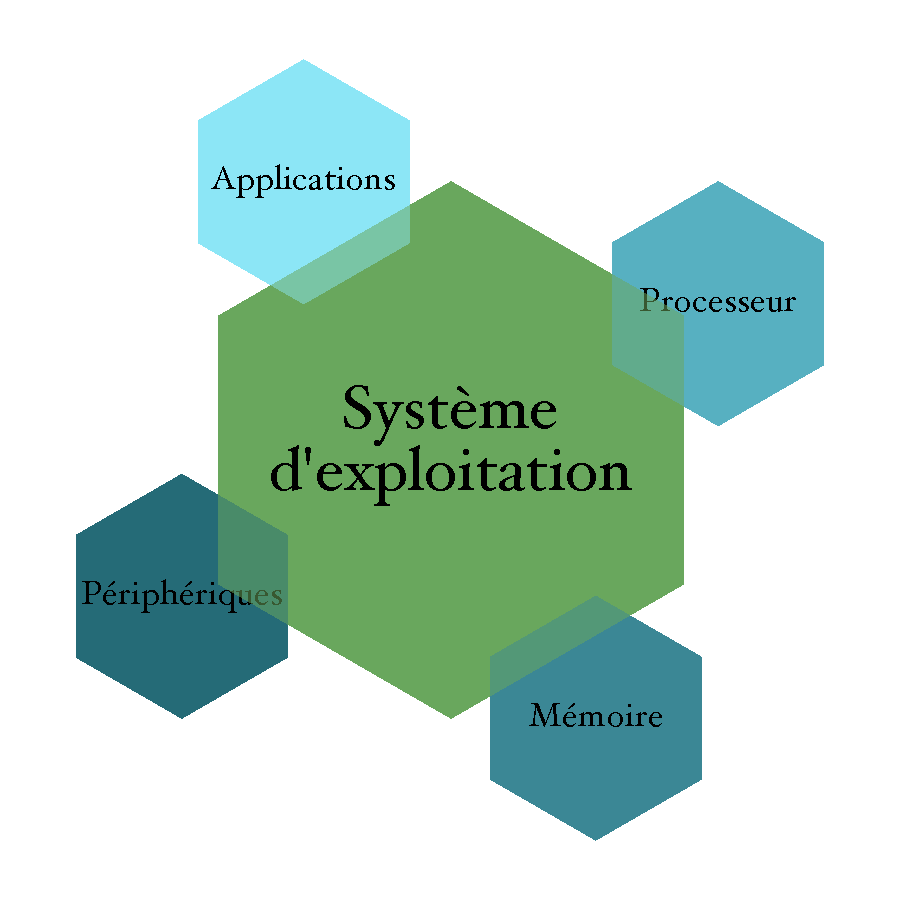
\includegraphics[scale=0.5]
  {textures/images/intro/os.pdf}
	\caption{Relations du système d'exploitation}
\end{figure}

Celui-ci est donc l'intermédiaire entre les logiciels, l'utilisateur et le
matériel (\textit{carte graphique, processeur, mémoire, périphériques, etc.}).
\\ Il gère ainsi la mémoire de l'ordinateur et la répartit entre tous les
programmes. \\ Par conséquent, lorsqu'une application nécessite diverses
informations, il lui suffit de faire appel au système d'exploitation.

\newpage

\subsection{Rôles}
Le système d'exploitation occupe différents rôles : \\

\begin{itemize}
\item \textbf{Gestion du processeur} : l'OS permet de gérer l'allocation du
processeur utile entre les différents programmes. \\

\item \textbf{Gestion de la mémoire vive} : celui-ci permet également
l'allocation de la mémoire utile afin de stocker les données des différentes
applications, ainsi que des différents utilisateurs. \\

\item \textbf{Gestion des entrées/sorties} (\textit{I/O}) : le système
d'exploitation permet de gérer les périphériques tels que des imprimantes,
scanneurs, souris, disques durs, etc. \\

\item \textbf{Gestion de l'exécution des applications} : il gère l'exécution
des applications et leur affecte les ressources nécessaires pour s'exécuter \\

\item \textbf{Gestion des droits} : le système d'exploitation s'assure que
l'application a des restrictions sur l'accès aux fichiers critiques (comme le
dossier \textit{System32} sous Windows) ainsi que les utilisateurs ne possédant
pas les droits adéquats (\textit{session invité}). \\

\item \textbf{Gestion des fichiers} : il gère la lecture ainsi que l'écriture
des fichiers et les droits d'accès aux fichiers par les logiciels et les
utilisateurs. \\

\item \textbf{Gestion des informations} : l'OS avertit l'utilisateur du bon
fonctionnement de l'ordinateur notamment à l'aide d'indicateurs et de logiciels
de diagnostic. \\

\item \textbf{Gestion de l'environnement de bureau} : le système affiche des
fenêtres et des icônes imitant un véritable bureau vu de haut
(\textit{calculatrice, corbeille, documents, ...}). Cette interface permet
d'utiliser facilement un ordinateur. Avant, tout se déroulait en ligne de
commande (\textit{CLI}) à l'aide d'un langage dédié. \\

\item \textbf{Gestion de la sécurité} : c'est à lui de veiller à la sécurité
d'agressions externes (réseau ou périphériques externes) ainsi qu'à la sécurité
de fonctionnement lors de pannes (logicielles ou matérielles). Le système doit
alors sauvegarder automatiquement les fichiers lors de l'arrêt et doit
permettre le redémarrage et la récupération des fichiers.
\end{itemize}

\newpage

\subsection{Différents systèmes d'exploitation}
Il existe un grand nombre de systèmes d’exploitation dédiés à différents
matériels (\textit{ordinateurs, smartphones et tablettes, cartes à puces,
véhicules, robots, équipement réseau, etc.}). \\

Chacun ayant une interface et des logiciels adaptés au matériel pour lequel il
est développé. \\ Les systèmes pour ordinateurs sont adaptés aux grands écrans
et à la navigation clavier-souris, alors que, pour le mobile, ils ont une
interface prévue pour le tactile et des écrans de plus petite taille. \\

Les deux familles de systèmes d'exploitation les plus populaires sont Unix
(principalement \textit{OS X, GNU/Linux, iOS et Android}) et Windows. Cette
dernière détient un quasi-monopole sur les ordinateurs personnels avec près de
90\% de part de marché depuis 15 ans. \\

Il est à noter que, depuis Windows 8, le système de Microsoft est adapté aux
tablettes et autres écrans tactiles (ce n’est pas le cas de Windows pour
smartphones qui est un autre OS nommé Windows Phone et Windows 10 Mobile). \\

Du côté de Apple, le système mobile (iOS anciennement \textit{iPhone OS}) est
un dérivé de Mac OS X. En effet, leur base est commune et leur plus grande
différence réside dans leur interface graphique. \\

Chez GNU/Linux, il existe un grand nombre de systèmes d’exploitation mobiles
(comme \textit{Android, Firefox OS, Tizen ou encore Ubuntu Touch}). \\
Android en est, de loin, le plus connu avec 85\% de part de marché dans le
mobile. \\

Pour les équipements réseau, il existe Cisco IOS qui s'utilise via la ligne
de commande. \\

De manière générale, il existe de nombreux systèmes d'exploitation portant
sur divers domaines. Ceux-ci sont développés pour une technologie bien précise
ce qui explique, entre autres, la multitude de ces OS dans le quotidien. \\
Bien entendu, pour les systèmes d'exploitation mobiles et ceux liés aux
ordinateurs, il y a des incompatibilités en terme de logiciels. Cela signifie
qu'un logiciel qui fonctionne sur un OS peut ne pas s'exécuter correctement sur
un autre.

\newpage

\subsection{Marché des OS}

Voici les parts de marché des systèmes d'exploitation les plus utilisés par
catégorie : \\

\begin{tabular} {p{7cm} p{8cm}}
	\begin{itemize}
  \item[$\bullet$] \textbf{Ordinateurs} (Janvier 2016) :
    \begin{enumerate}
    \item Windows (\textbf{85,18\%})
    \item Mac OS X (\textbf{9,03\%})
    \item GNU/Linux (\textbf{1,47\%})
    \item Chrome OS (\textbf{0,51\%})
    \item Autres (\textbf{3,81\%})
    \end{enumerate}
	\end{itemize}
	& \begin{itemize}
  \item[$\bullet$] \textbf{Smartphones et tablettes} (2014) :
    \begin{enumerate}
    \item Android (\textbf{85\%})
    \item iOS (\textbf{11\%})
    \item Windows Phone (\textbf{2,5\%})
    \item BlackBerry OS (\textbf{1\%})
    \item Autres (\textbf{0,5\%})
    \end{enumerate}
	\end{itemize}
\end{tabular}

En ne gardant que les trois systèmes les plus utilisés de chaque catégorie, on obtient ce classement:

\begin{center}
	\begin{tabular} {p{8cm}} \centering
		\begin{enumerate}
    \item Windows \textit{PC et Mobile} (\textbf{45,15\%})
    \item Android (\textbf{43,77\%})
    \item iOS (\textbf{5,66\%})
    \item Mac OS X (\textbf{4,66\%})
    \item Linux (\textbf{0,76\%})
		\end{enumerate}
	\end{tabular}
\end{center}

\begin{figure}[!h]
  \center
  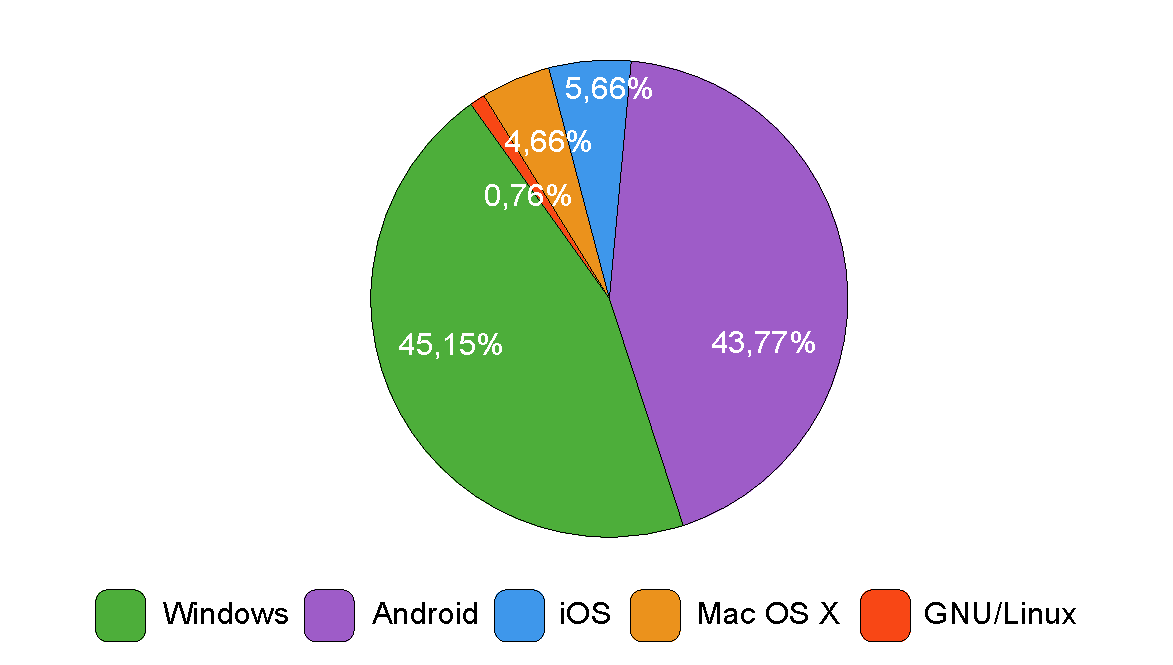
\includegraphics[scale=0.52]
  {textures/images/intro/moreUsedOS.pdf}
  \caption{Statistiques des systèmes d'exploitation plus utilisés}
\end{figure}

\newpage

Par conséquent, les cinq systèmes d'exploitation les plus utilisés sont, dans
l'ordre décroissant : Windows, Android, iOS, Mac OS X et GNU/Linux. \\

Il est à noter qu'aux USA, les parts de marché de Windows ont fortement baissé
en 8 ans : elles sont passées de près de 95\% à 20\%. \\ Microsoft se retrouve
maintenant derrière Google avec Android et Chrome OS (42\%) et Apple avec OS X
et iOS (24\%). \\

Logos de ces différents OS: \\

\begin{figure}[!h]
	\centering
	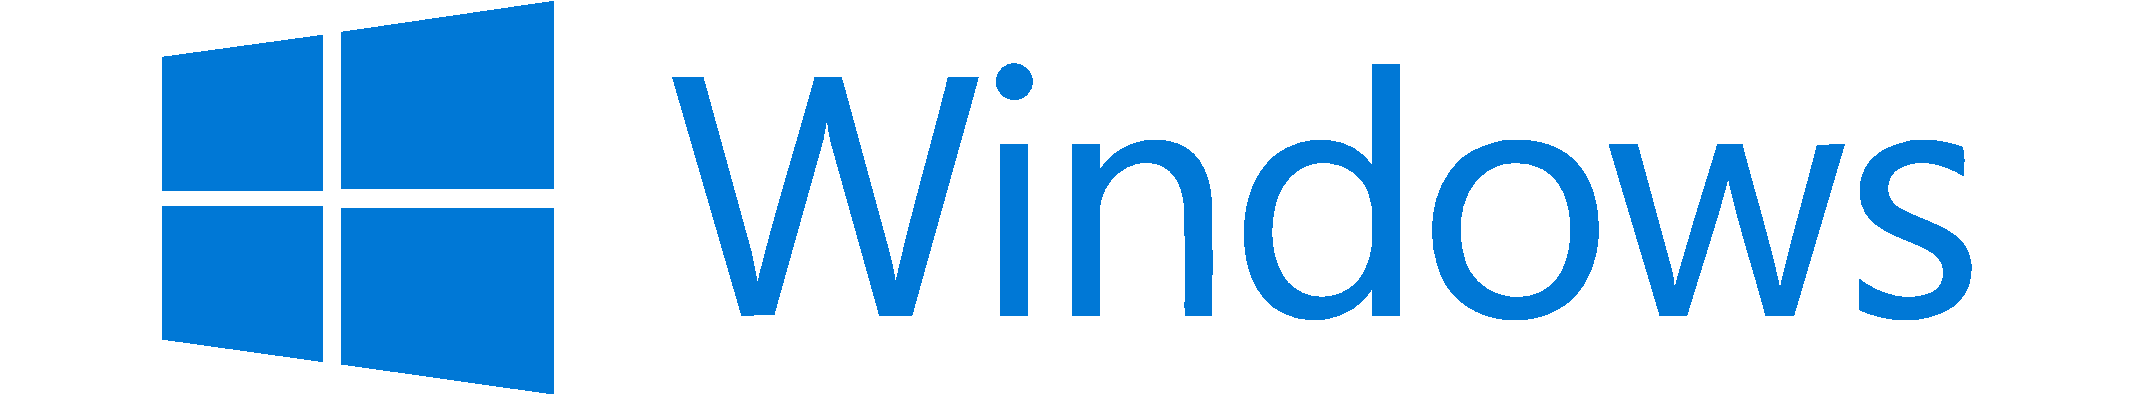
\includegraphics[scale=0.1]
	{textures/images/intro/logo/windows.pdf}
	\caption{Logo de Windows}
\end{figure}

\begin{figure}[!h]
	\centering
	
\includegraphics[scale=0.03]
	{textures/images/intro/logo/android.pdf}
	\caption{Bugdroid, la mascotte de Android}
\end{figure}

\begin{figure}[!h]
	\centering
	
\includegraphics[scale=0.03]
	{textures/images/intro/logo/ios.pdf}
	\caption{Logo de iOS}
\end{figure}

\begin{figure}[!h]
	\centering
	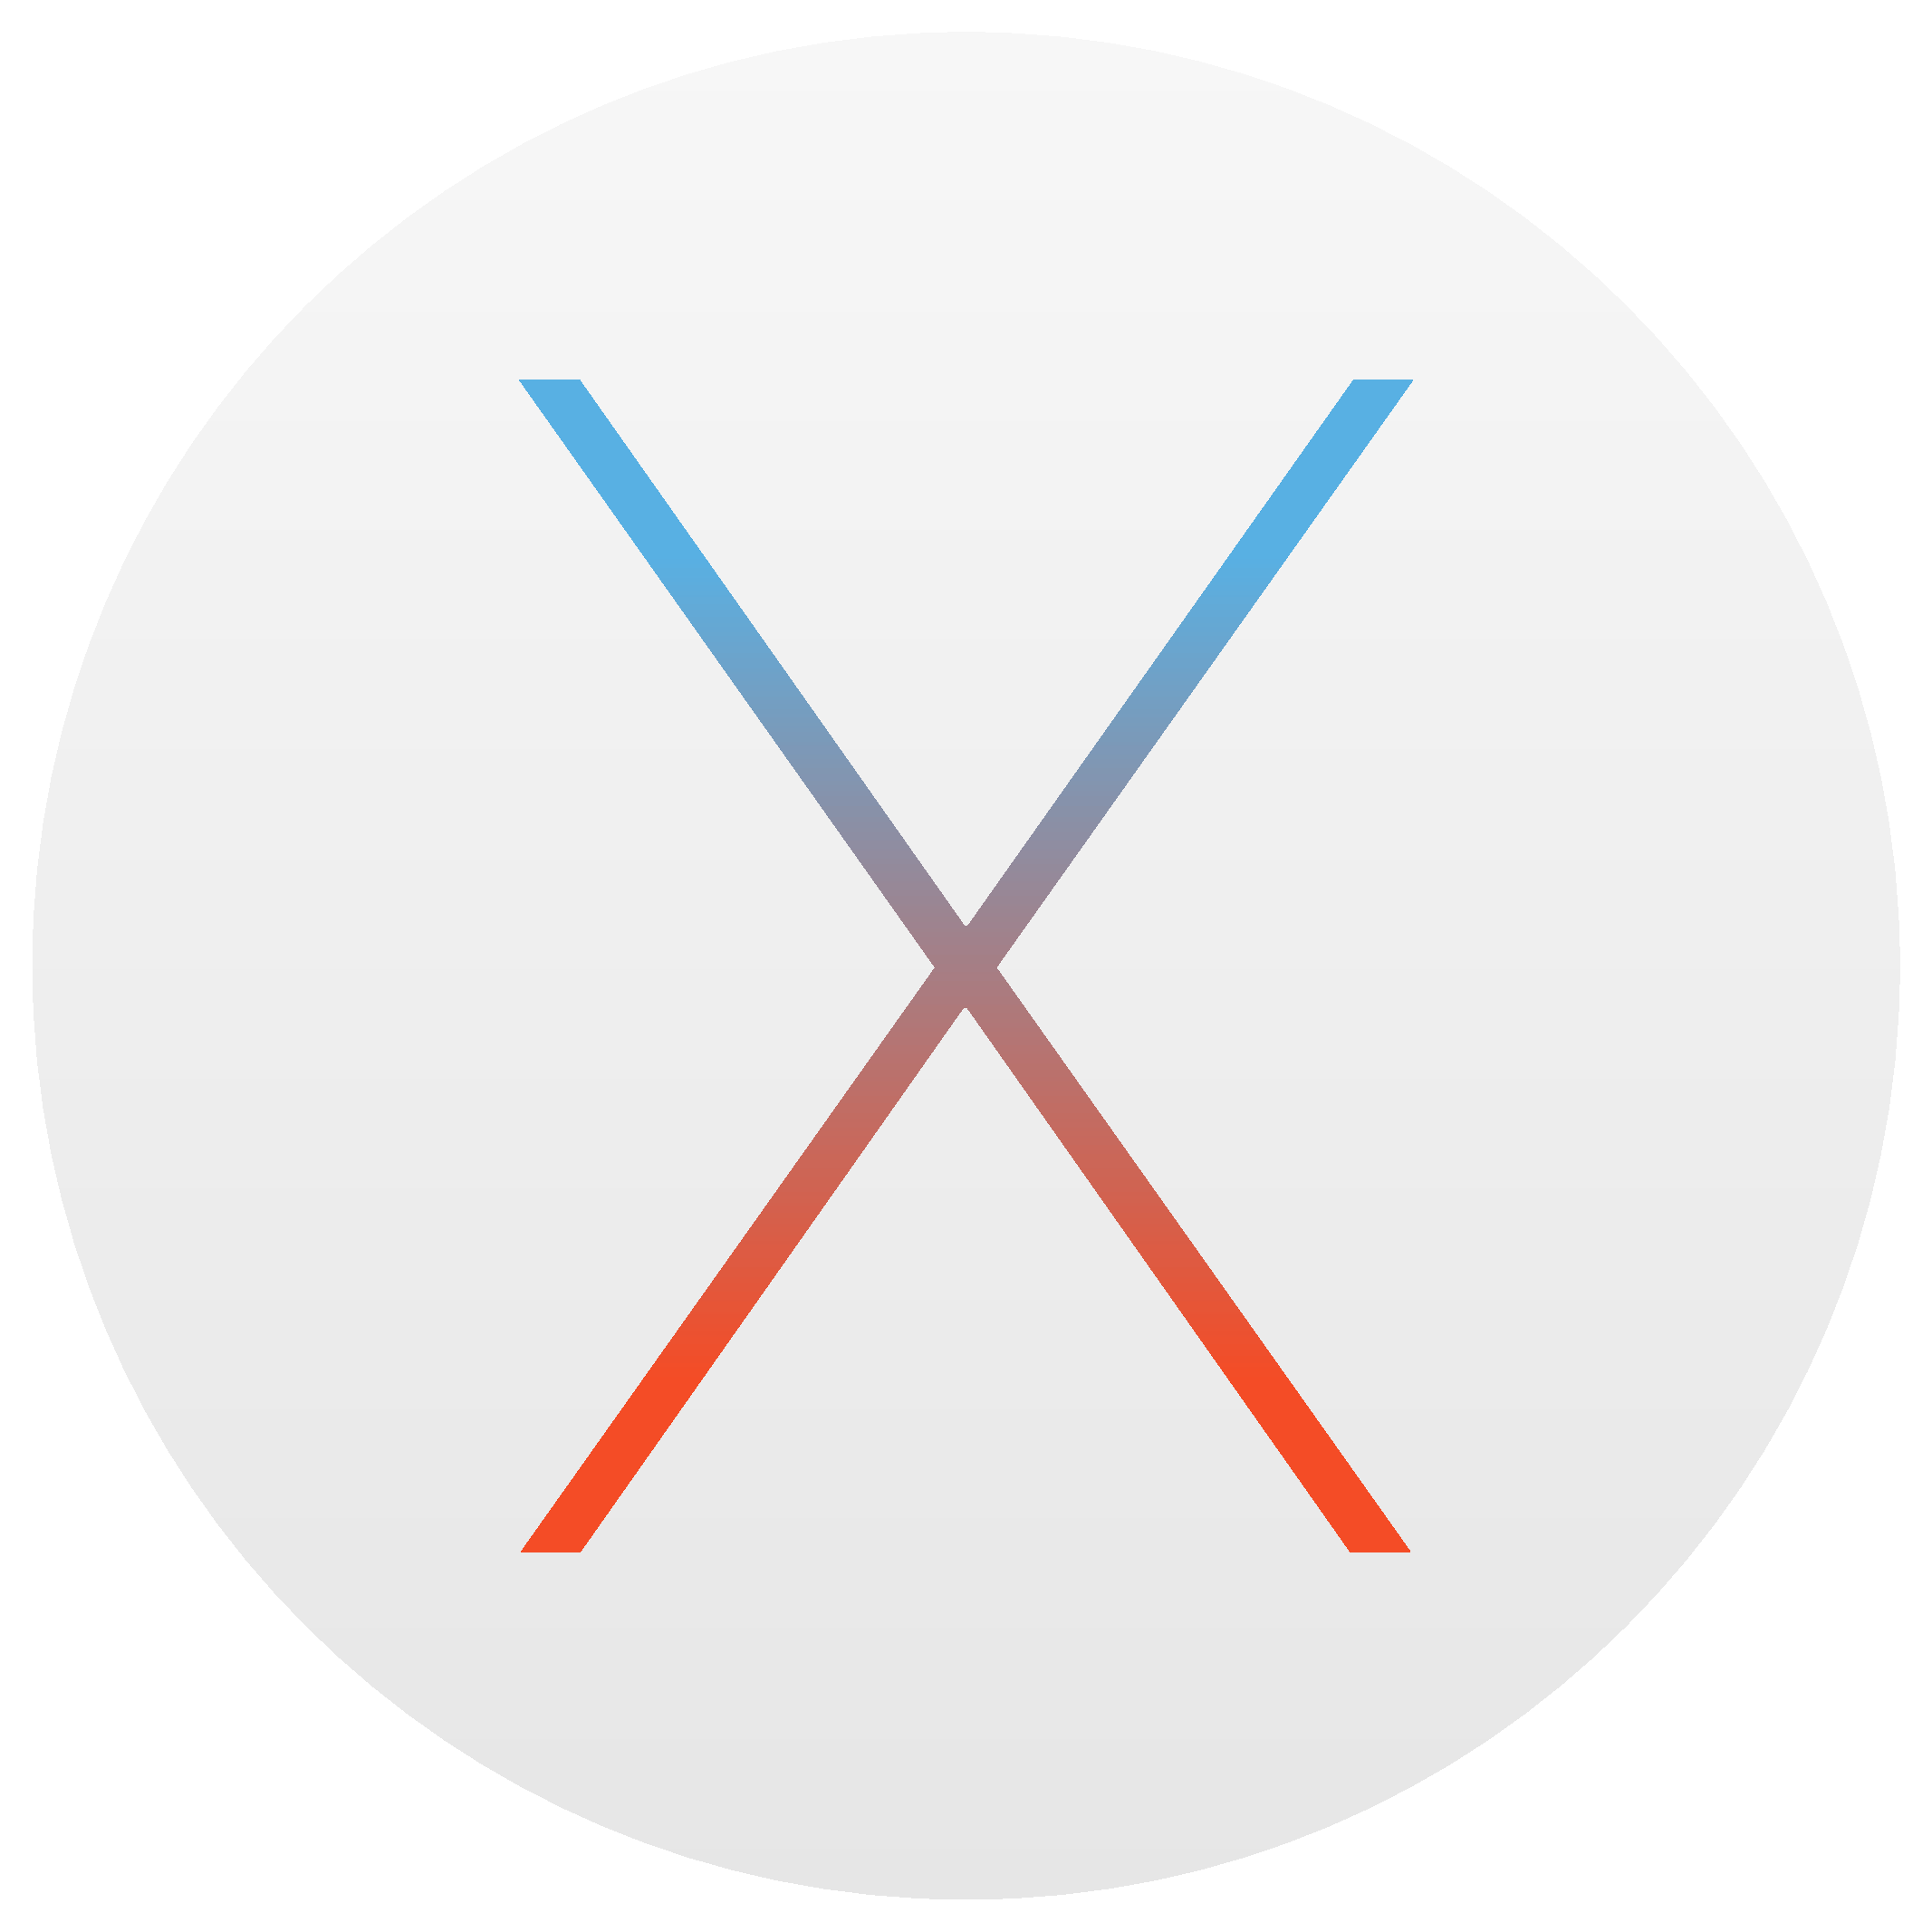
\includegraphics[scale=0.03]
	{textures/images/intro/logo/osx.pdf}
	\caption{Logo de Mac OS X}
\end{figure}

\begin{figure}[!h]
	\centering
	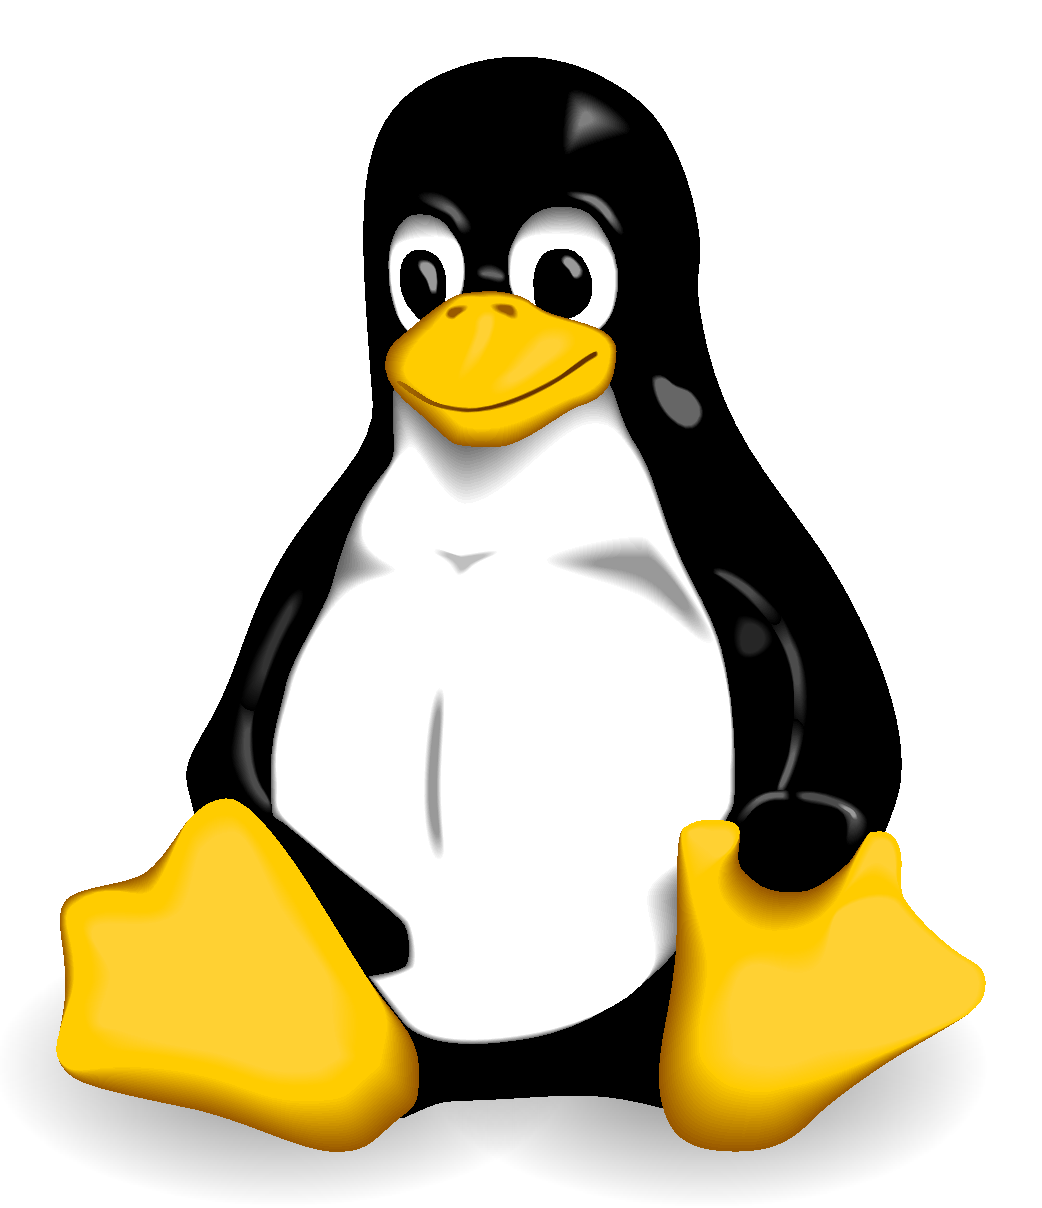
\includegraphics[scale=0.05]
	{textures/images/intro/logo/tux.pdf}
	\caption{Tux, la mascotte de Linux}
\end{figure}
